%%%%%%%%%%%%%%%%%%%%%%%%%%%%%%%%%%%%%%%%%%%
\newif\ifinclude		% if per l'include dei file
%\includetrue	

%%%%%%%%%%%%%%%%%%%%%%%%%%%%%%%%%%%%%%%%%%%
%
% Template per Elaborato di Laurea
% DISI - Dipartimento di Ingegneria e Scienza dell’Informazione
%
% update 2015-09-10
%
%%%%%%%%%%%%%%%%%%%%%%%%%%%%%%%%%%%%%%%%%%%

%%%%%%%%%%%%%%%%%%%%%%%%%%%%%%%%%%%%%%%%%%%

% formato FRONTE RETRO
\documentclass[epsfig,a4paper,11pt,titlepage,twoside,openany]{book}
\usepackage{epsfig}
\usepackage{plain}
\usepackage{setspace}
\usepackage[paperheight=29.7cm,paperwidth=21cm,outer=1.5cm,inner=2.5cm,top=2cm,bottom=2cm]{geometry} % per definizione layout
\usepackage{titlesec} % per formato custom dei titoli dei capitoli

\singlespacing

\usepackage[italian]{babel}

%%%%%%%%%%%%%%%%% STEFANO ADDED %%%%%%%%%%%%%%%%
% supporto lettere accentate
% queste due righe nel preambolo servono a poter utilizzare le lettere accentate in tutto il testo se no di norma si inserirebbero con \'e...
\usepackage[T1]{fontenc}
\usepackage[utf8]{inputenc}
\usepackage{hyperref} %Serve per i riferimenti
\usepackage{caption}  %Serve per le note (caption)
\usepackage{multicol}	 %Serve per usare più colonne

%%%%%%%%%%%%%%%%% ENRICO ADDED %%%%%%%%%%%%%%%%%
\usepackage{ulem} %Serve per il sottolineato
\usepackage{amsmath} %Serve per alcuni ambienti matematici
\usepackage{array} %Serve per le tabelle
\usepackage{multirow} %Seve per tabelle
\setcounter{secnumdepth}{5} %Utilissimo serve per aumentare il numero di paragrafi, si arriva fino a 5 livelli di profondità x.x.x.x.x
%GRAFICI
\usepackage{pgfplots}
\usepackage{pgfmath}
\usepackage{tikz}
%CODICE
% \usepackage{listings}
% \usepackage[cache=false]{minted} 
%\setminted{tabsize=4, breaklines, breakanywhere, linenos, mathescape,}

% \lstset{
% 	  breakatwhitespace=false,         
% 	  breaklines=true,     
% 	  basicstyle=\footnotesize\ttfamily,            
% 	  commentstyle=\color{blue}, %Indica il colore dei commenti
% 	  keywordstyle=\color{red}, %Indica il colore delle parole chiave
% 	  language=C, %Indica il linguaggio predefinito da usare
% 	  rulecolor=\color{black}, %Indica il colore dei numeri di righe
% 	  tabsize=4,
% 	  escapeinside={\%*}{*)},
% 	  morekeywords={}, %Altre parole da inserire tra le keywords. Ad esempio possiamo aggiungere do, gotttto, ecc ecc 
% }
%%%%%%%%%%%%%%%%% END OF ENRICO  %%%%%%%%%%%%%%%%

\begin{document}
%set the language of the text to italian
% !TeX spellcheck = it_IT

%%%%%%% personal commands (ALIAS):
% \newcommand{\nome_commando}[argomenti]{comando}
\newcommand{\e}[1]{$\cdot 10^{#1}$}
\newcommand{\mmax}[0]{mod\_withMax }
\newcommand{\mover}[0]{mod\_overlap }
\newcommand{\mmod}[0]{modularità modificata }
\newcommand{\nv}[0]{Node2Vec }
\newcommand{\wv}[0]{Word2Vec }
\newcommand{\cnrl}[0]{CNRL }
\newcommand{\cora}[0]{Cora }
\newcommand{\citeseer}[0]{Citeseer }
\newcommand{\LPred}[0]{Link Prediction }
%



	
 	% nessuna numerazione
	\ifinclude
  		\pagenumbering{gobble} 
  		\pagestyle{plain}

\thispagestyle{empty}

\begin{center}
	\begin{figure}[h!]
    	\centerline{
\psfig{file=immagini/logo_unitn_black_center.eps,width=0.6\textwidth}}
  	\end{figure}

  \vspace{2 cm} 

  \LARGE{Dipartimento di Ingegneria e Scienza dell’Informazione\\}

  \vspace{1 cm} 
  \Large{Corso di Laurea in\\
    Informatica\\
    %Informatica
    %Ingegneria dell'Informazione e delle Comunicazioni
    %Ingegneria dell'Informazione e Organizzazione d'Impresa
    %Ingegneria Elettronica e delle Telecomunicazioni    
  }
  \vspace{1 cm} 
  \Large{Percrso di studio\\
    Scienze e Tecnologie Informatiche 
  }
  	

  \vspace{2 cm} 
  \Large\textsc{Elaborato finale\\} 
  \vspace{1 cm} 
  \Huge\textsc{Titolo?\\}
  \Large{\it{Sottotitolo (alcune volte lungo - opzionale)?}}


  \vspace{2 cm} 
  \begin{tabular*}{\textwidth}{ c @{\extracolsep{\fill}} c }
  \Large{Supervisore} & \Large{Laureando}\\
  \Large{Alberto Montresor}& \Large{Stefano Leonardi}\\
  \end{tabular*}

  \vspace{2 cm} 

  \Large{Anno accademico 2017/2018}
  
\end{center}

  		\clearpage
  	 \fi
  
%%%%%%%%%%%%%%%%%%%%%%%%%%%%%%%%%%%%%%%%%%%
%% Nota: Sezione Ringraziamenti opzionale
  	\ifinclude
  		\thispagestyle{empty}

\begin{center}
  {\bf \Huge Ringraziamenti}
\end{center}

\vspace{2cm}
\noindent Ringrazio tutti coloro che in questi anni mi sono stati vicini, mi hanno motivato a crescere e a non mollare anche quando tutto è andato storto. Grazie a chi ha creduto in me, fino a che l'obbiettivo, da lontano e difficile, è diventato sempre più vicino e tangibile.\\
Ora che ho conquistato questo traguardo sono certo che sarà motivo di gioia ed orgoglio per i miei genitori, i parenti e gli amici tutti. Un grazie a tutti gli amici con cui ho condiviso la bellissima esperienza del mondo circense, da cui ho imparato a vivere col sorriso qualsiasi situazione. Altrettanto ringrazio gli amici di più vecchia data, che mi conoscono e m'accompagnano da molti anni.\\
Sono convinto che mi sarete tutti vicini anche per i progetti futuri a cui già sto pensando.\\
Un doveroso ringraziamento va poi a chi ha reso possibile questo lavoro di tesi, il dottorando Nasrullah Sheikh per la sua guida e al prof. Alberto Montresor per la pazienza e i preziosi consigli che mi sono stati di grande aiuto.

  		\clearpage
  		\pagestyle{plain} % nessuna intestazione e pie pagina con numero al centro
  	\fi

  \mainmatter % inizio numerazione pagine in numeri arabi

%%%%%%%%%%%%%%%%%%%%%%%%%%%%%%%%%%%%%%%%%%%
%% Nota:  Si ricorda che il numero massimo di facciate è 30.
%% Nel conteggio delle facciate sono incluse 
%%   indice
%%   sommario
%%   capitoli
%% Dal conteggio delle facciate sono escluse
%%   frontespizio
%%   ringraziamenti
%%   allegati    
%%%%%%%%%%%%%%%%%%%%%%%%%%%%%%%%%%%%%%%%%%%

    % indice
    \ifinclude
    	\tableofcontents
    	\clearpage
    \fi

    % gruppo per definizone di successione capitoli senza interruzione di pagina
    \begingroup
    
    % nessuna interruzione di pagina tra capitoli
    % ridefinizione dei comandi di clear page
    \renewcommand{\cleardoublepage}{} 
    \renewcommand{\clearpage}{} 
    
    % redefinizione del formato del titolo del capitolo
    % da formato
    %   Capitolo X
    %   Titolo capitolo
    % a formato
    %   X   Titolo capitolo
    \titleformat{\chapter}
    	{\normalfont\Huge\bfseries}{\thechapter}{1em}{}
    	
      	\titlespacing*{\chapter}{0pt}{0.59in}{0.02in}
      	\titlespacing*{\section}{0pt}{0.20in}{0.02in}
      	\titlespacing*{\subsection}{0pt}{0.10in}{0.02in}
      
	%\ifinclude
      	% sommario
      	%%%%%%%%%%%%%%%%%%%%%%%%%%%%%%%%%%%%%%%%%%%%

% formato FRONTE RETRO
\documentclass[epsfig,a4paper,11pt,titlepage,twoside,openany]{book}
\usepackage{epsfig}
\usepackage{plain}
\usepackage{setspace}
\usepackage[paperheight=29.7cm,paperwidth=21cm,outer=1.5cm,inner=2.5cm,top=2cm,bottom=2cm]{geometry} % per definizione layout
\usepackage{titlesec} % per formato custom dei titoli dei capitoli

\singlespacing

\usepackage[italian]{babel}

%%%%%%%%%%%%%%%%% STEFANO ADDED %%%%%%%%%%%%%%%%
% supporto lettere accentate
% queste due righe nel preambolo servono a poter utilizzare le lettere accentate in tutto il testo se no di norma si inserirebbero con \'e...
\usepackage[T1]{fontenc}
\usepackage[utf8]{inputenc}
\usepackage{hyperref} %Serve per i riferimenti
\usepackage{caption}  %Serve per le note (caption)
\usepackage{multicol}	 %Serve per usare più colonne

%%%%%%%%%%%%%%%%% ENRICO ADDED %%%%%%%%%%%%%%%%%
\usepackage{ulem} %Serve per il sottolineato
\usepackage{amsmath} %Serve per alcuni ambienti matematici
\usepackage{array} %Serve per le tabelle
\usepackage{multirow} %Seve per tabelle
\setcounter{secnumdepth}{5} %Utilissimo serve per aumentare il numero di paragrafi, si arriva fino a 5 livelli di profondità x.x.x.x.x
%GRAFICI
\usepackage{pgfplots}
\usepackage{pgfmath}
\usepackage{tikz}
%CODICE
% \usepackage{listings}
% \usepackage[cache=false]{minted} 
%\setminted{tabsize=4, breaklines, breakanywhere, linenos, mathescape,}

% \lstset{
% 	  breakatwhitespace=false,         
% 	  breaklines=true,     
% 	  basicstyle=\footnotesize\ttfamily,            
% 	  commentstyle=\color{blue}, %Indica il colore dei commenti
% 	  keywordstyle=\color{red}, %Indica il colore delle parole chiave
% 	  language=C, %Indica il linguaggio predefinito da usare
% 	  rulecolor=\color{black}, %Indica il colore dei numeri di righe
% 	  tabsize=4,
% 	  escapeinside={\%*}{*)},
% 	  morekeywords={}, %Altre parole da inserire tra le keywords. Ad esempio possiamo aggiungere do, gotttto, ecc ecc 
% }
%%%%%%%%%%%%%%%%% END OF ENRICO  %%%%%%%%%%%%%%%%

\begin{document}
%set the language of the text to italian
% !TeX spellcheck = it_IT

%%%%%%% personal commands (ALIAS):
% \newcommand{\nome_commando}[argomenti]{comando}
\newcommand{\e}[1]{$\cdot 10^{#1}$}
\newcommand{\mmax}[0]{mod\_withMax }
\newcommand{\mover}[0]{mod\_overlap }
\newcommand{\mmod}[0]{modularità modificata }
\newcommand{\nv}[0]{Node2Vec }
\newcommand{\wv}[0]{Word2Vec }
\newcommand{\cnrl}[0]{CNRL }
\newcommand{\cora}[0]{Cora }
\newcommand{\citeseer}[0]{Citeseer }
\newcommand{\LPred}[0]{Link Prediction }
%



%
%
\chapter{Sommario}
%% cos'è?
%% Il sommario è un breve riassunto del lavoro svolto dove si descrive: l’obiettivo, l’oggetto della tesi, le metodologie e le tecniche usate, i dati elaborati e la spiegazione delle conclusioni alle quali siete arrivati.
%% Il sommario dell’elaborato consiste al massimo di 3 pagine e deve contenere le seguenti informazioni: contesto e motivazioni breve riassunto del problema affrontato tecniche utilizzate e/o sviluppate risultati raggiunti, sottolineando il contributo personale del laureando/a se vi sono più persone che hanno contribuito...
Questa tesi va a ripercorrere il lavoro svolto da Leonardi Stefano durante il tirocinio svolto all'interno dell'università, con la supervisione del dottorando Sheikh Nasrullah, per il professore Montresor Alberto.
%
\section{Introduzione}
L'intero tirocinio è basato sull'articolo intitolato "Community-enhanced Network Representation Learning for Network Analysis" che può essere abbreviato con la sigla \cnrl. Questo articolo propone un innovativo metodo per individuare delle comunità all'interno dei grafi. Lo scopo di questo tirocinio è stato quindi quello di replicare i risultati ivi proposti, una volta compreso il codice alla base, e, dove possibile, cercare di migliorare le prestazioni dell'algoritmo proposto, anche sfruttando elementi non originariamente considerati.\newline
L'algoritmo proposto nell'articolo sfrutta diverse tecniche, alcune delle quali dettagliatamente spiegate negli articoli:
\begin{itemize}
	\item "DeepWalk: Online Learning of Social Representations"
	\item "node2vec: Scalable Feature Learning for Networks"
	\item "How exactly does word2vec work?"
\end{itemize} 
Di seguito la spiegazione del perché l'individuazione di comunità è una tecnica così importante.
%
\section{Cosa sono i grafi e cosa le comunità}
Alla base di tutto vi sono i grafi, una particolare struttura dati composta da nodi/vertici $V$ (dove $n=|V|$) e archi/bordi/lati $E$ (dove $m=|E|$). I primi possono rappresentare un entità eventualmente anche con l'aiuto di attributi. Diversamente gli archi sono dei collegamenti che legano due nodi, questi possono essere interamente orientati o non orientati. Questa struttura dati permette di rappresentare tantissime situazioni per tale motivo è così importante.\\
Lo scopo dell'individuazione di comunità è, come dice il nome, scovare delle comunità, ossia dei gruppi di nodi simili fra loro.\\
È importante notare che i nodi possono essere simili per molte diverse ragioni, possono avere le stesse caratteristiche strutturali in quanto sono dei cardini che legano molti altri elementi, magari dei punti isolati da tutto il resto, o più semplicemente hanno i valori di alcuni attributi analoghi.\\
Trovare nodi simili permette di gestirli in maniera omogenea e di sfruttarne le peculiarità. Visto che con i grafi possono rappresentare molte situazioni anche le comunità risultano essere molto versatili, per tale motivo sono tanto importanti.
%
\section{Come si valutano le comunità}
È stato spiegato cosa sono i grafi e cosa sono le comunità che vi si possono costruire sopra, ma non è stato spiegato come si può decidere, date due partizioni differenti su un grafo, quale di queste due è la migliore. Intuitivamente se il grafo è molto piccolo tanto da poterlo comprendere guardando unicamente una sua rappresentazione grafica, e le comunità individuate sono poche allora si potrebbe decidere anche ad occhio qual è la migliore partizione.\\
Se però le comunità individuate sono tante e il grafo non è più piccolo, allora non è più così facile effettuare una scelta e tanto meno riuscire a giustificarla. Esistono perciò dei metodi formali per analizzare e decidere cosa andare a preferire, questi metodi prendono il nome di modularità.\\
\\
Prima di parlare di ciò è però necessario formalizzare il concetto di partizione per comprendere di cosa si sta parlando:
\begin{itemize}
	\item Una partizione è un insieme di comunità
	\item Non tutte le comunità hanno le stesse dimensioni, ossia lo stesso numero di nodi che vi appartengono
	\item Le comunità non hanno né una dimensione massima né una dimensione minima.\\
	In realtà si può considerare che la loro dimensione cada nell'intervallo $[1, n]$, dove il limite inferiore $1$ è dato dal fatto che devono contenere almeno un elemento, mentre il limite superiore $n$ è dato dal fatto che non può contenere più nodi di quelli esistenti nel grafo (che sono in numero di $n$)
	\item È possibile che un nodo non appartenga a nessuna comunità
	\item Un nodo del grafo può appartenere a più di una comunità, potenzialmente anche a tutte quelle presenti, questo significa che c'è una sovrapposizione di comunità
\end{itemize}
Come accennato la metrica di valutazione di una partizione è la modularità (il cui simbolo è $Q$). Questo nome può essere associato a diverse metriche infatti a seconda di cosa cerchiamo avremo interesse a valorizzare certi aspetti e penalizzarne altri, per tale motivo la modularità è solo il nome usato per indicare la valutazione di una partizione.\\
Durante il tirocinio sono stati adottati tre metodi differenti: \mmax, \mover e \mmod. I primi due nomi non sono ufficiali in quanto sono stati scelti al solo scopo di riconoscerle, mentre l'ultimo \mmod è quello utilizzato nell'articolo su \cnrl .\\
I dettagli sul funzionamento e del perché le abbiamo scelte sono all'interno dell'apposito capitolo sulle metriche di valutazione.
%
\section{I cambiamenti apportati}
Per calcolare la partizione il codice di \cnrl utilizza un sistema di visite random e grazie a questo ricostruisce le possibili somiglianze fra i nodi. Non volendo toccare questa sezione le modifiche da noi riportate si inseriscono all'interno della creazione grazie a tali visite, dei cammini.\\
Una cammino è definito come una sequenza di nodi, preso un elemento qualsiasi fra questi deve esser possibile arrivare all'elemento successivo attraversando un solo arco, ossia i due elementi devono essere direttamente connessi, almeno nel senso di percorrenza.\\
L'algoritmo genera $x$ cammini, ognuno di lunghezza massima $l$, sul grafo, dove $x=n*w$:
\begin{itemize}
	\item $n$: è il numero di nodi del grafo
	\item $w$: è il numero di cammini che si fanno partire da ogni singolo nodo
	\item $l$: è la lunghezza massima di ogni cammino
\end{itemize}
%
Con questi dati l'algoritmo di \cnrl calcola la suddivisione in comunità, si può notare come tutti questi dati vengono estratti esclusivamente dalla struttura del grafo, ossia da come nodi ed archi sono interconnessi.\\
L'intuizione sfruttata per modificare l'algoritmo sta nel fatto che esistono altri dati non utilizzati, ossia gli attributi dei nodi. Tramite la creazione di nuovi particolari cammini è possibile far risultare due nodi in precedenza lontani, in quanto non direttamente connessi, vicini, in quanto questi due nodi condividono uno o più attributi. È facile intuire che l'introduzione di tutti questi nuovi dati porta ad un radicale cambiamento della suddivisione in comunità.
%
\section{Risultati}
Parte temporaneamente mancante...

%
%
%
%
\newpage
%\end{document}

 	%\fi
      
%%%%%%%%%%%%%%%%%%%%%%%%%%%%%%%%%%%%%%%%%%%
%% Nota:
%% Sommario e' un breve riassunto del lavoro svolto dove si descrive 
%% l’obiettivo, l’oggetto della tesi, le metodologie e 
%% le tecniche usate, i dati elaborati e la spiegazione delle conclusioni 
%% alle quali siete arrivati.
%% Il sommario dell’elaborato consiste al massimo di 3 pagine e deve contenere le seguenti informazioni: 
%%   contesto e motivazioni
%%   breve riassunto del problema affrontato
%%   tecniche utilizzate e/o sviluppate
%%   risultati raggiunti
%%%%%%%%%%%%%%%%%%%%%%%%%%%%%%%%%%%%%%%%%%% 
      
	%%%%%%%%%%%%%%%%%%%%%%%%%%%%%%%%
    % lista dei capitoli
    %
    % \input oppure \include
    %
    
    %%%%%%%%%%%%%%%%%%%%%%%%%%%%%%%%%%%%%%%%%%%%%

% formato FRONTE RETRO
\documentclass[epsfig,a4paper,11pt,titlepage,twoside,openany]{book}
\usepackage{epsfig}
\usepackage{plain}
\usepackage{setspace}
\usepackage[paperheight=29.7cm,paperwidth=21cm,outer=1.5cm,inner=2.5cm,top=2cm,bottom=2cm]{geometry} % per definizione layout
\usepackage{titlesec} % per formato custom dei titoli dei capitoli

\singlespacing

\usepackage[italian]{babel}

%%%%%%%%%%%%%%%%% STEFANO ADDED %%%%%%%%%%%%%%%%
% supporto lettere accentate
% queste due righe nel preambolo servono a poter utilizzare le lettere accentate in tutto il testo se no di norma si inserirebbero con \'e...
\usepackage[T1]{fontenc}
\usepackage[utf8]{inputenc}
\usepackage{hyperref} %Serve per i riferimenti
\usepackage{caption}  %Serve per le note (caption)
\usepackage{multicol}	 %Serve per usare più colonne

%%%%%%%%%%%%%%%%% ENRICO ADDED %%%%%%%%%%%%%%%%%
\usepackage{ulem} %Serve per il sottolineato
\usepackage{amsmath} %Serve per alcuni ambienti matematici
\usepackage{array} %Serve per le tabelle
\usepackage{multirow} %Seve per tabelle
\setcounter{secnumdepth}{5} %Utilissimo serve per aumentare il numero di paragrafi, si arriva fino a 5 livelli di profondità x.x.x.x.x
%GRAFICI
\usepackage{pgfplots}
\usepackage{pgfmath}
\usepackage{tikz}
%CODICE
% \usepackage{listings}
% \usepackage[cache=false]{minted} 
%\setminted{tabsize=4, breaklines, breakanywhere, linenos, mathescape,}

% \lstset{
% 	  breakatwhitespace=false,         
% 	  breaklines=true,     
% 	  basicstyle=\footnotesize\ttfamily,            
% 	  commentstyle=\color{blue}, %Indica il colore dei commenti
% 	  keywordstyle=\color{red}, %Indica il colore delle parole chiave
% 	  language=C, %Indica il linguaggio predefinito da usare
% 	  rulecolor=\color{black}, %Indica il colore dei numeri di righe
% 	  tabsize=4,
% 	  escapeinside={\%*}{*)},
% 	  morekeywords={}, %Altre parole da inserire tra le keywords. Ad esempio possiamo aggiungere do, gotttto, ecc ecc 
% }
%%%%%%%%%%%%%%%%% END OF ENRICO  %%%%%%%%%%%%%%%%

\begin{document}
%set the language of the text to italian
% !TeX spellcheck = it_IT

%%%%%%% personal commands (ALIAS):
% \newcommand{\nome_commando}[argomenti]{comando}
\newcommand{\e}[1]{$\cdot 10^{#1}$}
\newcommand{\mmax}[0]{mod\_withMax }
\newcommand{\mover}[0]{mod\_overlap }
\newcommand{\mmod}[0]{modularità modificata }
\newcommand{\nv}[0]{Node2Vec }
\newcommand{\wv}[0]{Word2Vec }
\newcommand{\cnrl}[0]{CNRL }
\newcommand{\cora}[0]{Cora }
\newcommand{\citeseer}[0]{Citeseer }
\newcommand{\LPred}[0]{Link Prediction }
%



%
%
\chapter{Implementation}
In this section, I am going to explain thanks to which method we tried to outperform the potentiality of the code of CNRL. 
\section{How the CNRL's code work}
How the code of CNRL exactly work?\\
First of all, the data are loaded from files, this includes the graph in edgelist format. After that, the graph is prepared for node2vec algorithm this is a particular method for exploring the graph, in fact, it depends on two parameters, named $p$ and $q$. The value of the two parameters allow a depth visit or something that are more similar to a breadth visit, or possibly a solution in the middle.\\
But why we walk on the graph?\\
The main idea is to start some walks (in the number of $w$), from each node of the graph (in the number of $n$). And each walk have a length not higher than the value of $l$, I said not higher because if we have a directed graph it is possible that we arrive in a sink, then the walk must be interrupted because it is not possible to walk more. Differently, if we have an undirected graph all the walks have a length of $l$ because node2vec allows a path that goes back.\\
At the end of that, we have $w \cdot n$ walks with a maximum length of $l$\\
Given the walks it is possible to obtain the community of the graph, this process is done with two different approaches, the first one is one of the most famous, named word2vec, that is going to consider the nodes' ID find in the walks like words, and then consider the walks like sentences.\\
Differently in the code of CNRL is used an algorithm created on purpose, and we have never tried to understand how it works exactly.\\
After that the partition is created, it is possible to calculate the modularity, with the algorithm that I explained in his chapter.
%
\section{Introduce of attribute}
As you can understand, CNRL's code for calculating the community use only the structure of the graph, that means, how the nodes and the edges are interconnected.\\
We note that both dataset on which we work, named Cora and Citeseer (better explained in the chapter on the experiments), have for each node a set of attribute, this can be present 1 or not 0. All those pieces of information are not considered from the CNRL's code so we decide to introduce it. The only part where we can work is before the extraction of the community given the walks and after the loading of data from the input files, this means that we can change only the generation of the walks.\\
The idea is to create in addition to the firsts walks, some other walks that manage the nodes through the attributes. When we see at the graph we can say that two nodes are near if there is a link between them.\\
When can we say that two nodes through an attribute are similar? Of course, when both share the same attribute. We can imagine that the sharing of an attribute is like an undirected link or edge, in fact, there is not any direction with the sharing. Then we can build a new undirected graph that considers the attribute and we are going to go to walk on it.
%
\section{Attribute graph}
In all the previous words we have described the graph taken from the attribute. I try now to formalize this concept.\\
First of all, we must remember that we have the original edges that we must delete, in fact, we do not want to walk on it, or the new walks will be a copy of the first ones. Then from the original graph, we preserve only the nodes, called from now N1.\\
Thanks to the reasoning done before, that if two nodes share the same attribute, they are near. We can imagine that an edge, goes or directly from a node of N1 to another. Or we can create a new set of nodes, named N2, that contain all the attributes, each attribute becomes a node.
%
\begin{figure}[htp]
	\centering
	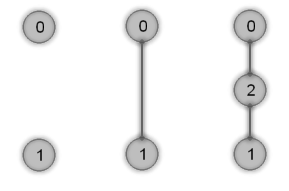
\includegraphics{images/add_att2}
	\caption{Two nodes that share an attribute, how we can link them, 1-no edge, 2-hypergraph, 3-bipartite graph}
	\label{fig:add_att2}
\end{figure}
\begin{figure}[htp]
	\centering
	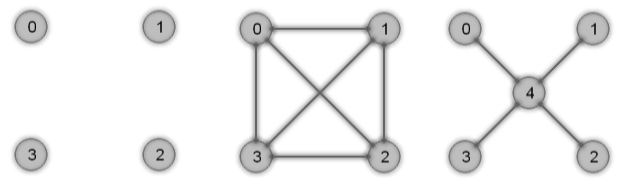
\includegraphics[width=\linewidth]{images/add_att4}
	\caption{Four nodes that share an attribute, how we can link them, 1-no edge, 2-hypergraph, 3-bipartite graph}
	\label{fig:add_att4}
\end{figure}
\\
Then exist two methods to link some nodes through the attribute. In figure~\ref{fig:add_att2} and~\ref{fig:add_att4}, there are two different examples. In both figures we have three scenes, the first one shows the nodes without any linkage, the second one shows the nodes connected directly, in the last one we have the nodes connected across another node that does the hub, this hub is the node taken from the attribute.
Is easy to understand the difference, the second scene, named hypergraph, create a complete graph, this mean that I have  $ \displaystyle\binom{n}{2}$ edges, in figure~\ref{fig:add_att4} are $ \displaystyle\binom{4}{2} = 6$, but no one node is added.\\
The third scene is a star graph that builds a bipartite graph, add a node for each attribute, but only $n$ edges, for figure~\ref{fig:add_att4} this mean that we add one node and four edges.\\
Which one we prefer?\\
It depends on the situations, if there are lots of attributes and each of these is available for a little number of nodes, probably we are going to prefer the hypergraph. If there are some attribute that is available for a high number of nodes probably we prefer the bipartite graph.\\
In fact if for example we have an attribute available for $100$ nodes this mean that with the bipartite graph we add $1$ node and $100$ edges, for the hypergraph we add zero nodes but $ \displaystyle\binom{100}{2} = 4950$ edges.\\
For this reason, we have chosen for use the bipartite graph.\\
To note that when we walk on this new graph we save in the array of walks for both type of nodes, then after walking we must delete the ID of the nodes belonging to the attributes. Because the future steps of the algorithm must not know the existence of the bipartite graph.
%
\subsection{Name of bipartite graph}
I would like to explain where this name does come from. The graph is called bipartite because there are two set of nodes, the nodes that before I called N1 (original nodes) and N2 (nodes from attribute). Every edge of the graph goes from a node of N1 to a node of N2 and vice versa. There is no one edge that goes from N1 to N1 or from N2 to N2. This is perfect for our situation if we had two nodes of N1 linked this would mean that we have not deleted the original edges if we would have two nodes of N2 linked this would mean that we have done an error, two attributes can not be linked.
%
\subsection{Name of hypergraph}
I would like to explain where this name does come from. The hypergraph do not have simple edges but have hyperedges, the normal edges have two endpoints and both are nodes, so its possible to represent it with a line. Differently, the hyperedges do not have two endpoints but potentially an infinite number of endpoints, this allows that a hyperedge link more than two nodes directly. If you want to represent an hyperedges on a normal undirected graph this mean that, if the hyperedges link directly 5 nodes we must replace it with a complete graph on this 5 nodes so we use $ \displaystyle\binom{5}{2} = 10$ normal edges.

Note that, this is exactly our situation, in fact, an attribute link the nodes to which it belongs directly, so we can imagine that for each attribute we are going to create a hyperedge on his nodes.
%
%

\section{Build graph - example}
In this section, I am going to show how a graph is transformed from the simple structure and the attributes to a hypergraph or to a bipartite graph.\\
%
\begin{multicols}{2}
	\begin{center}
		\begin{tabular}{|l|cc|}
		\hline
		ID&\multicolumn{2}{c|}{attributes ID}\\
		\hline
		1&11&\\
		2&11&12\\
		3&10&12\\
		4&11&13\\
		5&11&12\\
		6&12&13\\
		7&13&14\\
		\hline
		\end{tabular}
		\captionof{table}{For each node, there are the attributes ID that it has}
		\label{tab:7_ID_to_att}
		%
		\begin{tabular}{|l|cccc|}
		\hline
		att&\multicolumn{4}{c|}{node ID}\\
		\hline
		10&3&&&\\
		11&1&2&4&5\\
		12&2&3&5&6\\
		13&4&6&7&\\
		14&7&&&\\
		\hline
		\end{tabular}
		\label{tab:7_att_to_ID}
		\captionof{table}{For each attribute, there are the nodes ID that it has}
	\end{center}
\end{multicols}
%
%
\begin{figure}[htp]
	\centering
	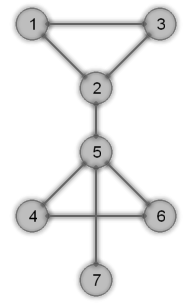
\includegraphics{images/7transform_str}
	\caption{The structure representation of the graph}
	\label{fig:7transform_str}
\end{figure}
%
%
In figure~\ref{fig:7transform_str} we can see the structure of the graph. In table~\ref{tab:7_ID_to_att} we can see that for each node is represented the ID of the attributes that it has. At the opposite in table~\ref{tab:7_att_to_ID} for each attribute, are represented the ID of the nodes that have it.\\
Then now it is possible to create the two graphs.
%
\begin{figure}[htp]
	\centering
	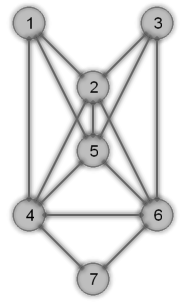
\includegraphics{images/7transform_hyper}
	\caption{The representation of the hypergraph}
	\label{fig:7transform_hyper}
\end{figure}
\\
First, we look at the hypergraph shown in figure~\ref{fig:7transform_hyper}.
\begin{itemize}
	\item  we can see that some edges are no more present, two examples are $(1,3)$ and $(5,7)$, some other before was deleted and after they are replaced
	\item  the nodes that share the same attribute build a complete graph, two example are $[1,2,4,5]$ with the attribute $11$ and $[4,6,7]$ with the attribute $13$
	\item  if only one node has a particular attribute this does not create an edge, this is the case of the two attributes $10$ and $14$
\end{itemize}
%
\begin{figure}[htp]
	\centering
	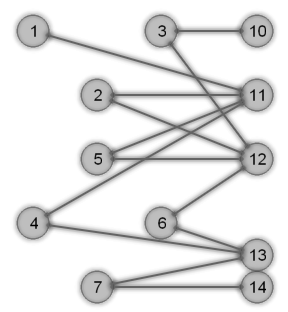
\includegraphics{images/7transform_bipartite}
	\caption{The representation of the bipartite graph}
	\label{fig:7transform_bipartite}
\end{figure}
%
We look now a more complex situation, the bipartite graph shown in figure~\ref{fig:7transform_bipartite}. It is not easy to see what happen.\\
The nodes from 1 to 7, on the left, are the original ones the nodes from 10 to 14 (higher equal than 10), on the right, are the new ones created from the attributes. 
\begin{itemize}
	\item the nodes on the left and the nodes on the right are separate are the two sets of which I spoke before N1 and N2
	\item all edges cross the middle of the graph, go from left to right
	\item all the edges present in the original graph are no more present, we have deleted all of them
	\item the nodes that share the same attribute build a star graph, two example are $[1,2,4,5]$ with the attribute $11$ and $[4,6,7]$ with the attribute $13$
	\item  if only one node has a particular attribute this do not do difference, in fact, the two attributes $10$ and $14$ are anyway linked to the left part
\end{itemize}
%
%
%
%\end{document}
		%capitolo 1
    %%%%%%%%%%%%%%%%%%%%%%%%%%%%%%%%%%%%%%%%%%%%%

% formato FRONTE RETRO
\documentclass[epsfig,a4paper,11pt,titlepage,twoside,openany]{book}
\usepackage{epsfig}
\usepackage{plain}
\usepackage{setspace}
\usepackage[paperheight=29.7cm,paperwidth=21cm,outer=1.5cm,inner=2.5cm,top=2cm,bottom=2cm]{geometry} % per definizione layout
\usepackage{titlesec} % per formato custom dei titoli dei capitoli

\singlespacing

\usepackage[italian]{babel}

%%%%%%%%%%%%%%%%% STEFANO ADDED %%%%%%%%%%%%%%%%
% supporto lettere accentate
% queste due righe nel preambolo servono a poter utilizzare le lettere accentate in tutto il testo se no di norma si inserirebbero con \'e...
\usepackage[T1]{fontenc}
\usepackage[utf8]{inputenc}
\usepackage{hyperref} %Serve per i riferimenti
\usepackage{caption}  %Serve per le note (caption)
\usepackage{multicol}	 %Serve per usare più colonne

%%%%%%%%%%%%%%%%% ENRICO ADDED %%%%%%%%%%%%%%%%%
\usepackage{ulem} %Serve per il sottolineato
\usepackage{amsmath} %Serve per alcuni ambienti matematici
\usepackage{array} %Serve per le tabelle
\usepackage{multirow} %Seve per tabelle
\setcounter{secnumdepth}{5} %Utilissimo serve per aumentare il numero di paragrafi, si arriva fino a 5 livelli di profondità x.x.x.x.x
%GRAFICI
\usepackage{pgfplots}
\usepackage{pgfmath}
\usepackage{tikz}
%CODICE
% \usepackage{listings}
% \usepackage[cache=false]{minted} 
%\setminted{tabsize=4, breaklines, breakanywhere, linenos, mathescape,}

% \lstset{
% 	  breakatwhitespace=false,         
% 	  breaklines=true,     
% 	  basicstyle=\footnotesize\ttfamily,            
% 	  commentstyle=\color{blue}, %Indica il colore dei commenti
% 	  keywordstyle=\color{red}, %Indica il colore delle parole chiave
% 	  language=C, %Indica il linguaggio predefinito da usare
% 	  rulecolor=\color{black}, %Indica il colore dei numeri di righe
% 	  tabsize=4,
% 	  escapeinside={\%*}{*)},
% 	  morekeywords={}, %Altre parole da inserire tra le keywords. Ad esempio possiamo aggiungere do, gotttto, ecc ecc 
% }
%%%%%%%%%%%%%%%%% END OF ENRICO  %%%%%%%%%%%%%%%%

\begin{document}
%set the language of the text to italian
% !TeX spellcheck = it_IT

%%%%%%% personal commands (ALIAS):
% \newcommand{\nome_commando}[argomenti]{comando}
\newcommand{\e}[1]{$\cdot 10^{#1}$}
\newcommand{\mmax}[0]{mod\_withMax }
\newcommand{\mover}[0]{mod\_overlap }
\newcommand{\mmod}[0]{modularità modificata }
\newcommand{\nv}[0]{Node2Vec }
\newcommand{\wv}[0]{Word2Vec }
\newcommand{\cnrl}[0]{CNRL }
\newcommand{\cora}[0]{Cora }
\newcommand{\citeseer}[0]{Citeseer }
\newcommand{\LPred}[0]{Link Prediction }
%



%
\chapter{Metodi di valutazione}
Questo capitolo spiega di come si valuta una partizione creata dagli algoritmi d'individuazione delle comunità. Come citato nel sommario, il metodo scelto nel corso del tirocinio è stato la modularità, il cui simbolo è $Q$.\\
La modularità altro non è che un valore solitamente compreso all'interno dell'intervallo $[-1, 1]$. Tuttavia questo non è sempre vero poiché dipende strettamente da quale metodo d'implementazione si va ad utilizzare. Le prime persone che hanno lavorato sulla modularità sono state Newman e Girvan , che necessitavano di un metodo formale per decidere fra due partizioni di nodi quale fosse la migliore.\\
Newman e Girvan  quando hanno scritto le prime applicazioni della modularità sono partiti da una semplice assunzione: un nodo non può appartenere a più di una comunità. Questo elimina tutti i problemi dovuti alla sovrapposizione delle comunità. Per i casi studiati durante il tirocinio quest'assunzione non sempre è valida. Inizialmente è molto comoda poiché permette di ridurre notevolmente la complessità del calcolo della modularità.\\
\\
Durante tutto il lavoro svolto si è passati attraverso tre differenti metodi, tutti e tre verranno ora mostrati ed ove possibile spiegati, si parte dal più semplice fino ad arrivare al più complesso.\\ Durante la spiegazione di ogni metodo viene assunto di lavorare con grafi non orientati, alla fine di ogni sezione sono indicati gli eventuali cambiamenti da applicare in caso si abbia invece a che fare con grafi orientati.
%
\section{Modularità con massimi ( \mmax )}
È stato scelto questo nome in quanto questo metodo gestisce al massimo una comunità per ogni nodo, andando a ricalcare l'assunzione base di Newman e Girvan .\\
L'idea di base è che questo metodo va a calcolare un valore di modularità per ogni comunità. Tutti questi elementi sono poi sommati fra loro per andare a creare il valore di modularità del grafo in se. È necessario far notare che questo metodo non permette la sovrapposizione delle comunità, per l'assunzione fatta, di conseguenza è impossibile che la sommatoria finale vada a considerare più di una volta i valori raccolti, da un qualsiasi elemento del grafo.\\
Questo metodo si basa sull'osservazione che è possibile identificare una comunità sulla base della frequenza degli archi contenuti al suo interno. Di fatto se un insieme di nodi dispone di una grande quantità di archi che li collegano direttamente, questi nodi dovrebbero essere una comunità a sé stante o almeno far parte della stessa. Se così non fosse allora la valutazione della partizione sul grafo deve essere penalizzata in quanto non ha considerato questi nodi come parte dello stesso gruppo.\\
Il motivo per cui è stato scelto questo metodo, oltre al fatto che è semplice da calcolare, è proprio perché va a penalizzare le partizioni che non considerano una comunità molto evidente.\\
Di seguito la formula completa:
\begin{equation}
	Q=\sum_{c}^{C_r} \left( \frac{l_c}{L}-\left(\frac{d_c}{2L} \right)^2 \right)
	\label{eq:m_max}
\end{equation}
Dove gli elementi dell'equazione sono:
\begin{itemize}
	\item $Q$ è il simbolo di modularità
	\item $C_r$ è l'insieme delle comunità calcolate
	\item $c$ è l'iteratore sulle comunità
	\item $L$ è il numero totale di archi all'interno del grafo, solitamente indicato con $m=|E|$
	\item $l_c$ è il numero totale di archi interni alla comunità $c$, questo significa che ognuno degli archi qui contati ha ambo i nodi alle estremità appartenenti alla comunità $c$
	\item $d_c$ è il grado della comunità $c$, definito come la sommatoria dei gradi dei nodi che vi appartengono
\end{itemize}
%
Si può notare che $\frac{l_c}{L}$ è il peso della comunità $c$ rispetto al resto del grafo, in quanto si calcola la percentuale di archi di cui la comunità $c$ dispone. Mentre $\frac{d_c}{2L}$ è la densità di archi tramite cui la comunità $c$ interagisce, ossia quanto, rispetto al totale, sono importanti i nodi che appartengono a questa comunità.\\
\\
Quando si parla di grafo orientato l'unica parte da modificare è $\frac{d_c}{2L}$ che diventa $\frac{d_c}{L}$. In un grafo non orientato un arco incrementa di uno il grado di due nodi, quello  di partenza e quello d'arrivo, mentre, se l'arco fosse orientato questo non accadrebbe in quanto aumenterebbe solamente il grado del nodo di partenza, ecco il motivo del fattore moltiplicativo $2$ di differenza.
%
%
\section{Modularità con sovrapposizione ( \mover )}
L'algoritmo qui descritto è preso dall'articolo intitolato "Modularity measure of networks with overlapping communities"\cite{M-over_paper}.\\
Come si può intuire dal nome questo metodo permette a due comunità di condividere uno o più nodi e quindi d'aver una sovrapposizione. In linea con diversi altri metodi la modularità generata da questo algoritmo cade nell'intervallo $[-1, 1]$.\\
Se nel metodo precedente si calcolava un valore di modularità per ogni comunità e poi li si sommava in quanto non era prevista la sovrapposizione, qui la gestione è simile. Si calcola un valore per ogni comunità e poi, invece di sommarli, se ne ricava una media poiché la sovrapposizione è concessa. Uno stesso nodo può portare il suo contributo a diversi elementi della sommatoria.\\
Di seguito la formula completa:
\begin{equation}
	Q = M^{ov} = \frac{1}{K} 
	\sum_{r=1}^{K} \left[
		\frac
			{\sum\limits_{i \in c_r} 
				\left( \frac
					{
						\sum\limits_{j \in c_r, i \neq j} \left( a_{ij} \right) 
						- 
						\sum\limits_{j \notin c_r} \left( a_{ij} \right) 
					} 
					{d_i \cdot s_i} 
				\right) } 
			{n_{c_r}}
		\cdot
		\frac{ n^e_{c_r} }{ \binom{n_{c_r}}{2} } 
	\right]
	\label{eq:m_over}
\end{equation}
Dove gli elementi dell'equazione sono:
\begin{itemize}
	\item $C_r$ è l'insieme delle comunità calcolate
	\item $K$ è il numero di comunità calcolate, pari a $|C_r|$
	\item $c_r$ è la comunità attuale
	\item $n_{c_r}$ rappresenta il numero di nodi interni alla comunità $c_r$
	\item $n^e_{c_r}$ rappresenta il numero di archi interni alla comunità $c_r$
	\item $\binom{n_{c_r}}{2}$ è il numero massimo di archi potenzialmente presenti nella comunità $c_r$
	\item $d_i$ è il grado del nodo $i$
	\item $s_i$ è il numero di comunità a cui il nodo $i$ appartiene
	\item $a_{ij}$ vale 1 se l'arco dal nodo $i$ al nodo $j$ esiste, altrimenti assume il valore 0
\end{itemize}
%
Ecco spiegati dettagli presenti all'interno di quest'Equazione~\ref{eq:m_over}.\\
Come per il metodo precedente si calcola la densità della comunità (attraverso la Formula~\ref{eq:edge_density}). Ora si confronta il numero di archi interni presenti, rispetto al potenziale numero massimo, ossia il numero di archi presenti in un grafo completo con lo stesso numero di nodi.
\begin{equation}
	\frac{ n^e_{c_r} }{ \binom{n_{c_r}}{2} }
	\label{eq:edge_density}
\end{equation}
%
In aggiunta, si considera la relazione fra il numero di archi interni e quelli uscenti (tramite la Formula~\ref{eq:in-out_edge_relation}). Di conseguenza sembrerebbe che se il numero di archi uscenti è maggiore rispetto al numero di archi interni il valore di modularità vada ad assumere un valore negativo, in caso contrario positivo.\\
\begin{equation}
	\sum\limits_{i \in c_r} \left( \frac{
		\sum\limits_{j \in c_r, i \neq j} \left( a_{ij} \right) - 
		\sum\limits_{j \notin c_r} \left( a_{ij} \right) 
	} {d_i \cdot s_i} \right)
	\label{eq:in-out_edge_relation}
\end{equation}
In realtà non è sempre così, si deve tener conto anche del peso degli elementi $d_i$ e $s_i$. Questi due parametri hanno il compito di assegnare ad ogni arco un valore rappresentativo della sua importanza, interno o uscente è completamente indifferente. Si può notare come il valore di un arco possa variare all'interno dell'intervallo $]0, 1]$. Un arco ha inizialmente valore $1$ e viene poi diviso per due interi positivi moltiplicati fra loro, in seguito viene considerato con peso positivo se favorisce la comunità ossia se è interno, negativo se così non è.\\
$d_i$ è importante perché va a premiare gli archi che partono da un nodo con un basso grado. Il nodo avendo pochi archi, fa si che ognuno di questi sia molto importante, in quanto, la somma totale dei pesi degli archi di un nodo, è un valore costante uguale per tutti i nodi. Inoltre, tramite $s_i$, si premiano i nodi che appartengono a poche comunità, poiché tali nodi meglio rappresentano la loro comunità d'appartenenza. Se un nodo è comune a tutte le comunità del grafo non è per nulla rappresentativo e quindi ogni volta avrà un influenza estremamente bassa.\\
\\
È stato scelto questo metodo poiché permette la sovrapposizione di comunità. Inoltre andando a calcolare un valore di modularità per ogni comunità individuata nel grafo si può facilmente capire quale di queste dà un maggior contributo al risultato finale e quale invece tende solo a penalizzare la partizione a causa della sua bassa coesione.\\
Compresa la formula generatrice, si può notare che un particolare valore di modularità può rivelare  due importanti dettagli del grafo:
\begin{itemize}
	\item un valore negativo sta a significare che i gruppi di nodi non sono densamente connessi al loro interno ma piuttosto legati a punti esterni. Pur con un valore negativo è possibile che gli archi interni siano in numero maggiore rispetto agli archi verso l'esterno, ma, se ciò accade, è perché i parametri di $d_i$ e $s_i$ hanno dato maggior rilevanza agli archi uscenti
	\item se la modularità ha un valore, che in assoluto si avvicina molto allo zero, sta a significare che il grafo valutato è estremamente sparso. Il fattore moltiplicativo mostrato nell'Equazione~\ref{eq:edge_density} va a collassare i vari elementi della formula vicino allo zero, di conseguenza anche la sommatoria non si allontanerà di molto da quel valore
\end{itemize}
Quando si parla di grafo orientato l'unica differenza, da considerare, la si applica alla Formula~\ref{eq:edge_density}. Si dà il caso che il numero massimo di archi in un grafo orientato sia il doppio del numero di archi per lo stesso grafo non orientato, questo per il semplice motivo che si possono creare due archi leganti gli stessi due nodi se presentano versi opposti. Pertanto il numero massimo cambia da $\binom{n_{c_r}}{2}$ per diventare $ 2\binom{n_{c_r}}{2}$.
%
%
\section{Modularità modificata}
Questo algoritmo\cite{M-mod_code} è preso dall'articolo intitolato "Incorporating Implicit Link Preference Into Overlapping Community Detection"\cite{M-mod_paper}.\\
Questo è l'algoritmo che è stato scelto da chi ha scritto l'articolo di \cnrl e, per questa ragione, è stato adottato anche da noi. È estremamente importante perché permette di replicare i risultati illustrati nel documento cui facciamo riferimento. Si ha quindi un punto fisso da cui partire e con cui all'occorrenza confrontarsi.\\
Sfortunatamente questo è il più lento dei tre metodi che vengono illustrati in questo capitolo, per il semplice motivo che è il più complesso, sia logicamente che computazionalmente.\\
Di seguito vi sono due versioni della stessa formula (senza sistema~\ref{eq:m_mod} e con sistema~\ref{eq:m_mod_system}):
\begin{equation}
	Q = \frac{1}{M} \cdot \sum_{u,v \in V}
		\left[
			\left( A \left[ u,v \right] - \frac{ d_{in}\left(u\right) \cdot d_{out}\left(v\right) }{M} \right)
			\cdot
			|C_u \cap C_v| 
		\right]
	\label{eq:m_mod}
\end{equation}
%
\begin{equation}
	Q = \frac{1}{M} \cdot \sum_{u,v \in V}
		\begin{cases}
			\begin{array}{ll}
				0 & |C_u \cap C_v| = 0 \\
				\left[ \left( A \left[ u,v \right] - \frac{ d_{in}\left(u\right) \cdot d_{out}\left(v\right) }{M} \right) \cdot |C_u \cap C_v| \right]
				& altrimenti
			\end{array}
		\end{cases}
	\label{eq:m_mod_system}
\end{equation}
Dove gli elementi delle equazioni sono:
\begin{itemize}
	\item $M$ può assumere due valori a seconda che il grafo sia orientato o no, ossia misura $m$ se indiretto assume invece il valore $2m$ se diretto.\\
	In tutto questo $m$ è il numero di archi del grafo, ossia come di norma $m=|E|$
	\item $u,v$ sono gli iteratori sui nodi del grafo, chiamati come di consueto $V$
	\item $A \left[ u,v \right]$ rappresenta il peso assunto dall'arco $(u, v)$. Se tale arco non esiste il valore è $0$, mentre se l'arco esiste il peso è un valore positivo, di default $1$
	\item $d_{in}\left(u\right)$ e $d_{out}\left(u\right)$ sono i gradi entranti e uscenti del nodo $u$, questi rispettivamente contano il numero di archi entranti e uscenti dal nodo.\\
	Se il grafo è indiretto, questi due valori, preso un qualsiasi nodo, saranno perfettamente uguali
	\item $C_u$ è l'insieme delle comunità a cui il nodo $u$ appartiene
	\item $|C_u \cap C_v|$ è il numero totale di comunità condivise fra i nodi $u$ e $v$
\end{itemize}
%
Come per i metodi precedenti segue una spiegazione delle varie sezioni di tale Formula~\ref{eq:m_mod}.\\
Si prende l'elemento $ |C_u \cap C_v|$: questo fattore moltiplicativo ci permette d'ignorare gli archi che legano nodi che non condividono nessuna comunità. Per capire il suo scopo si può pensare ad una partizione che non presenta sovrapposizioni, in questo caso tale componente permetterà di ignorare tutti gli archi che non sono interni ad una singola comunità, ma passano da una all'altra. Ignorando ora l'assunzione base di Newman e Girvan  si può dire che gli unici archi considerati sono quelli che rimangono interni ad almeno una comunità, anche se è permesso loro essere di collegamento fra altre. Il funzionamento di questo componente è illustrato bene nella seconda versione (Formula~\ref{eq:m_mod_system}), grazie al sistema si nota che se la condizione è verificata si può ignorare tutta la prima parte.\\
Oltre a filtrare gli archi utilizzabili questo componente assegna un importanza maggiore a quegli archi che connettono nodi che condividono molte comunità.
\begin{equation}
	\frac{ d_{in}\left(u\right) \cdot d_{out}\left(v\right) }{M}
	\label{eq:d_in-out}
\end{equation}
La base che si ignora o moltiplica è un valore positivo, se l'arco esiste (questo grazie ad $ A \left[ u,v \right]$), mentre assume un valore negativo se l'arco non c'è, in quanto al peso $0$ dell'arco inesistente si sottrae il fattore definito nella Formula~\ref{eq:d_in-out}.\\
Quest'espressione rappresenta la rilevanza di un arco, indipendentemente dalla sua esistenza. Se tale arco collega due nodi con gradi elevati risulta essere uno fra molti e quindi ha un'importanza limitata, se diversamente collega nodi con gradi bassi allora assume molta più importanza perché è un caso isolato e quindi prezioso.
%\end{document}



	%capitolo 2
    
    %\input{capitolo3}	%capitolo 3
    %\input{capitolo4}	%capitolo 4
    \endgroup


    % bibliografia in formato bibtex
    % aggiunta del capitolo nell'indice
    \addcontentsline{toc}{chapter}{Bibliografia}
    % stile con ordinamento alfabetico in funzione degli autori
    \bibliographystyle{plain}
    \ifinclude
    	\bibliography{biblio}
    \fi
%%%%%%%%%%%%%%%%%%%%%%%%%%%%%%%%%%%%%%%%%%%
%% Nota:
%%
%% Nella bibliografia devono essere riportati tutte le fonti consultate 
%% per lo svolgimento della tesi. La bibliografia deve essere redatta 
%% in ordine alfabetico sul cognome del primo autore. 
%% 
%% La forma della citazione bibliografica va inserita secondo la fonte utilizzata:
%% 
%% LIBRI
%% Cognome e iniziale del nome autore/autori, la data di edizione, titolo, casa editrice, eventuale numero dell’edizione. 
%% 
%% ARTICOLI DI RIVISTA
%% Cognome e iniziale del nome autore/autori, titolo articolo, titolo rivista, volume, numero, numero di pagine.
%% 
%% ARTICOLI DI CONFERENZA
%% Cognome e iniziale del nome autore/autori (anno), titolo articolo, titolo conferenza, luogo della conferenza (città e paese), date della conferenza, numero di pagine. 
%% 
%% SITOGRAFIA
%% La sitografia contiene un elenco di indirizzi Web consultati e disposti in ordine alfabetico. 
%% E’ necessario:
%%   Copiare la URL (l’indirizzo web) specifica della pagina consultata
%%   Se disponibile, indicare il cognome e nome dell’autore, il titolo ed eventuale sottotitolo del testo
%%   Se disponibile, inserire la data di ultima consultazione della risorsa (gg/mm/aaaa).    
%%%%%%%%%%%%%%%%%%%%%%%%%%%%%%%%%%%%%%%%%%%
%%%%%%%%%%%%%%%%%%%%%%%%%%%%%%%%%%%%%%%%%%%    

    \titleformat{\chapter}
        {\normalfont\Huge\bfseries}{Allegato \thechapter}{1em}{}
    % sezione Allegati - opzionale
    \appendix
    %\input{allegati}

\end{document}
